\documentclass[10pt, pdf, xcolor=pdftex, dvipsnames, table]{beamer}

%\usepackage[brazil]{babel}
\usepackage[english]{babel}
\usepackage[utf8]{inputenc}
\usepackage[T1]{fontenc}
\usepackage{amsfonts}
\usepackage{amsmath}
\usepackage{algorithm}
\usepackage{algpseudocode}
\usepackage{pgfpages}
\usepackage{fancyvrb}
\usepackage{times}
\usepackage{amsmath,amssymb}
\usepackage{graphicx}
\usepackage{hyperref}
\usepackage{pxfonts,txfonts}
\usepackage{url}
\usefonttheme{structurebold}
\usepackage{hyphenat}
\usepackage{multicol}
\usepackage{palatino}
\usepackage[normalem]{ulem}
\usepackage{booktabs}
\useunder{\uline}{\ul}{}
\usepackage{appendix}
\usepackage{float}
\usepackage{verbatim}
\usepackage{cooltooltips}
\usepackage{paralist}
\usepackage[inline]{enumitem}
\usepackage{multirow}
\usepackage{array}
\usepackage{xargs}
\usepackage{xcolor}
\usepackage{subfigure}
\usepackage{caption}
%\usepackage{bm}

\captionsetup{font=scriptsize,labelfont=scriptsize}
\captionsetup{skip=1pt,belowskip=1pt}

\definecolor{mygray}{gray}{0.8}

\newtheorem{hipotese}{Hipótese}

\usepackage{listings} % para inserir codigo fonte
\lstset{extendedchars=true,frame=tb,basicstyle=\footnotesize,stringstyle=\ttfamily,showstringspaces=true}

\renewcommand{\lstlistingname}{Listagem}

\newcommand{\x}{\textbf{\textcolor{Green}{$\surd$}}}
\newcommand{\xx}{\textbf{\textcolor{Blue}{$\odot$}}}
\newcommand{\xxx}{\textbf{\textcolor{Red}{$\times$}}}

\usetheme{Amsterdam}
\usefonttheme[onlymath]{serif}

\floatname{algorithm}{Algoritmo}

%\newenvironment<>{varblock}[2][.9\textwidth]{%
%\setlength{\textwidth}{#1}
%	\begin{actionenv}#3%
%    		\def\insertblocktitle{#2}%
%    		\par%
%    		\usebeamertemplate{block begin}}
%  		{\par%
%    		\usebeamertemplate{block end}%
%  	\end{actionenv}}

% Efeitos:
\transdissolve %dissolve a lamina anterior;
% \transsplitverticalout % a proxima lamina se abre como uma cortina no sentido horizontal;
% \transblindshorizontal % a lamina anterior converte-se linha a linha.

% Para gerar apenas as páginas sem efeitos de overlay use (bom para imprimir):
% \usepackage[handout]{beamer}

% Para colocar número de páginas no slide:
%\setbeamertemplate{footline}[frame number]

% Para retirar a barra de navegação:
\setbeamertemplate{navigation symbols}{}

% inserir logotipo a apresentação
\pgfdeclareimage[height=1.5cm]{logo}{images/lups_oficial.png}
\logo{\pgfuseimage{logo}}

% Ativa ou desativa as anotações
\setbeameroption{hide notes}
%\setbeameroption{show notes}

%==================================================================================

%EVENTO
%\renewcommand{\evento}{Apresentação de artigo - Metodologia para pesquisa e desenvolvimento em Computação }

% TITULO DA APRESENTACAO
\title{Mobility-Aware Application Scheduling in Fog Computing}

%Autor
\author{Luiz F. Bittencourt %$^{1}$
\and Javier Diaz-Montes %$^{1}$
\and Rajkumar Buyya %$^{2}$
\and Omer F. Rana
\and Manish Parashar
\newline
\newline
\and Presenter: Maicon Ança dos Santos
}

%%%%%%%%%%%%%%%%%%%%%%%%%%%%%%%%%%%%%%%%
% Instituição , 
%%%%%%%%%%%%%%%%%%%%%%%%%%%%%%%%%%%%%%%%

%\institute{1\quad Department of Computer Engineering, University of Science and Culture, Tehran, Iran \\ 2\quad School of Computer Engineering, Iran University of Science and Technology, Tehran, Iran
%}

%\date{\today}

\begin{document}

\frame{\titlepage}
\pgfdeclareimage[height=0.7cm]{logo}{images/lups_timbre.png}
\logo{\pgfuseimage{logo}}
%\frame{\tableofcontents}


%%%%%%%%%%%%%%%%%%%%%%%%%%%%%%%%%%%%%%%%%%%%%
% Conteúdo da Apresentação
%%%%%%%%%%%%%%%%%%%%%%%%%%%%%%%%%%%%%%%%%%%%%

\section[Introduction]{Introduction}

%\begin{frame}
%	\tableofcontents[currentsection]
%\end{frame}

\begin{frame}
	\frametitle{Introduction}
 	\begin{block}{}
 		\begin{itemize}
 			\item With new levels of computing capacity provides by Fog computing, new forms of resource allocation and management can be developed;
 			\newline
 		    \item The grow of the number of devices scattered and connected to Internet, producing and consuming data, requires a scalable resource management at unprecedented levels - focus on IoT.
 		\end{itemize}
 	\end{block}
\end{frame}

\begin{frame}
	\frametitle{Introduction}
 	\begin{block}{}
 		\begin{itemize}
 			\item Data also are produced at the edge. Data generation and consumption can occur at many differents places and times;
 			\newline
 		    \item Different applications can have different requirements, especially in terms of response time;
 		    \newline
 		    \item 
 		\end{itemize}
 	\end{block}
\end{frame}

%\begin{frame}
% 	\begin{figure}[htbp]
% 		\centerline{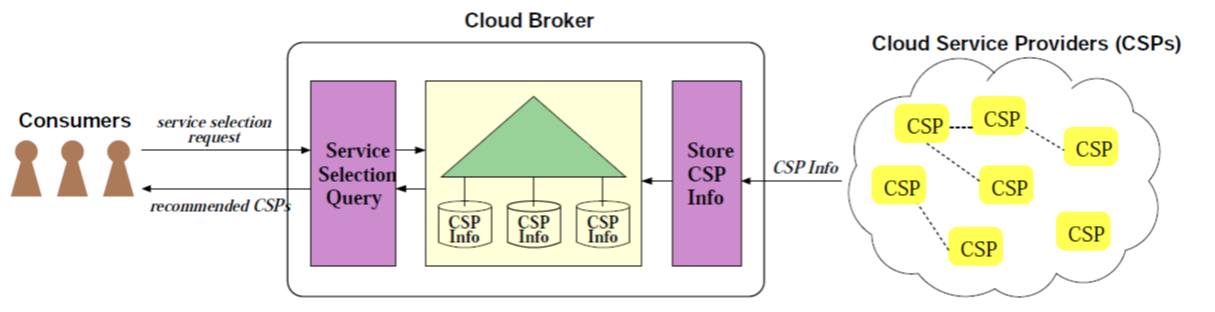
\includegraphics[scale=0.27]{images/CSBv2.png}}
% 		\caption[An Overview of the Cloud Broker Service]{An Overview of the Cloud Broker Service}
% 	\end{figure}
%\end{frame}

\begin{frame}
	\frametitle{Introduction}
 	\begin{block}{The problem}
 			\textit{Resource allocation considering the hierarchical infrastructure composed of edge capacity and cloud data centers, analyzing application classes along with different scheduling policies.}
 	\end{block}
\end{frame}

\section[Fog Computing Model]{Fog Computing Model}

\begin{frame}
	\tableofcontents[currentsection]
\end{frame}

\begin{frame}
	\frametitle{Fog Computing Model}
% 	\begin{block}{}
% 		\begin{itemize}
% 		    \item[•] Suporte para vários atributos de QoS
% 		    	\begin{itemize}
% 		    		\item[-] \footnotesize\textit{disponibilidade, segurança, desempenho, escalabilidade, confiabilidade}
% 		    	\end{itemize}
% 		    \item
% 		    \item[•] Reconhecimento de violação de SLA
% 		    	\begin{itemize}
% 		    		\item[-] \footnotesize\textit{identificar violações, tomar as medidas adequadas e compensar prejuízos acumulados.}
% 		    	\end{itemize}
% 		    \item
% 		    \item[•] Otimização de preços:
% 		    	\begin{itemize}
% 		    		\item[-] \footnotesize\textit{vial na decisão, os CSBs devem considerar importante na seleção.}
% 		    	\end{itemize}
% 		\end{itemize}
% 	\end{block}
\end{frame}

\begin{frame}
	\frametitle{Fog Computing Model}
% 	\begin{block}{}
% 		\begin{itemize}
% 		    \item[•] Seleção de fornecedores adequados para diferentes tipos de
% serviços na nuvem
% 				\begin{itemize}
% 		    		\item[-] \footnotesize\textit{everything as a service (XaaS); o CSB deve conhecer e pesquisar em todos}
% 		    	\end{itemize}
% 		    \item
% 		    \item[•] Perfil do cliente
% 		    	\begin{itemize}
% 		    		\item[-] \footnotesize\textit{problema de pesquisa: perfil ou histórico de solicitações acelera o processo }
% 		    	\end{itemize}
% 		    \item
% 		    \item[•] Corretagem dinâmica
% 		    	\begin{itemize}
% 		    		\item[-] \footnotesize\textit{O CSB deve selecionar o melhor serviço em função da dinâmica}
% 		    	\end{itemize} 
% 		\end{itemize}
% 	\end{block}
\end{frame}

\begin{frame}
	\frametitle{Fog Computing Model}
% 	\begin{block}{}
% 		\begin{itemize}
% 		    \item[•] Pedido parcial de informação sobre especificação de serviços
% dos clientes
% 				\begin{itemize}
% 		    		\item[-] \footnotesize\textit{os CSBs devem mediar entre os provedores e clientes menos profissionais}
% 		    	\end{itemize}
% 		    \item
% 		    \item[•] Priorização de preferência do cliente
% 		    	\begin{itemize}
% 		    		\item[-] \footnotesize\textit{as prioridades dos clientes devem ser consideradas na seleção dos serviços}
% 		    	\end{itemize}
% 		\end{itemize}
% 	\end{block}
\end{frame}

\section[Related Work]{Related Work}

\begin{frame}
	\tableofcontents[currentsection]
\end{frame}

\begin{frame}
	\frametitle{Related Work}
% 	\begin{block}{}
% 		\begin{itemize}
% 		    \item[•] Single service model
% 				\begin{itemize}
% 		    		\item[-] \footnotesize\textit{suportam o modelo de serviço SaaS, mas pode suportar outros modelos}
% 		    	\end{itemize}
% 		    \item
% 		    \item[•] Multiple service model
% 		    	\begin{itemize}
% 		    		\item[-] \footnotesize\textit{suportam mais de um modelo de serviço em nuvem: flexibilidade}
% 		    	\end{itemize}
% 		\end{itemize}
% 	\end{block}
\end{frame}

\begin{frame}
	\frametitle{Related Work}
% 	\begin{table}[]
% 		\centering
% 		\caption{Classificação de CSBs revisados}
% 		\label{my-label}
% 		\resizebox{\textwidth}{!}{%
% 		\begin{tabular}{cc}
% 			\hline
% 			\textbf{Single service model} & \textbf{Multiple service model} \\ \hline
% QBROKAGE & AHP \& TOPSIS \\
% SLA-based SaaS Provisioning & CSP-index \\
% Brokering Using Game Theory & Two Layered Brokerage \\
% STRATOS & SMICloud \\
% Distributed Cloud Brokering & Brokering for Optimized Placement of Virtual Machines \\
% Multi-Cloud Brokering & OWL-S Based Semantic CSB \\
% Dynamic Brokering on Federated Clouds & Price Optimization using 0-1 Knapsack \\
% T-Broker &  \\ \hline
% 		\end{tabular}%
% 	}
% 	\end{table}
\end{frame}

\section[Applications]{Applications}

\begin{frame}
	\tableofcontents[currentsection]
\end{frame}

\begin{frame}
	\frametitle{Applications}
% 	\begin{block}{}
% 		\begin{itemize}
% 		    \item[•] Não há suporte para vários modelos de serviço em nuvem:
% 				\begin{itemize}
% 		    		\item[-] \footnotesize\textit{o CSB deve ser capaz de encontrar provedores adequados para todos os tipos de serviço}
% 		    	\end{itemize}
% 		    \item
% 		    \item[•] Nenhum suporte desejável para atributos de QoS
% 		    	\begin{itemize}
% 		    		\item[-] \footnotesize\textit{o CSB deve suportar todos os atributos de QoS no momento da seleção do serviço}
% 		    	\end{itemize}
% 		\end{itemize}
% 	\end{block}
\end{frame}

\begin{frame}

\end{frame}

\begin{frame}

\end{frame}

\section[Allocation Policies]{Allocation Policies}

\begin{frame}
	\tableofcontents[currentsection]
\end{frame}

\begin{frame}
\end{frame}

\begin{frame}
 	\begin{figure}[htbp]
 		\centerline{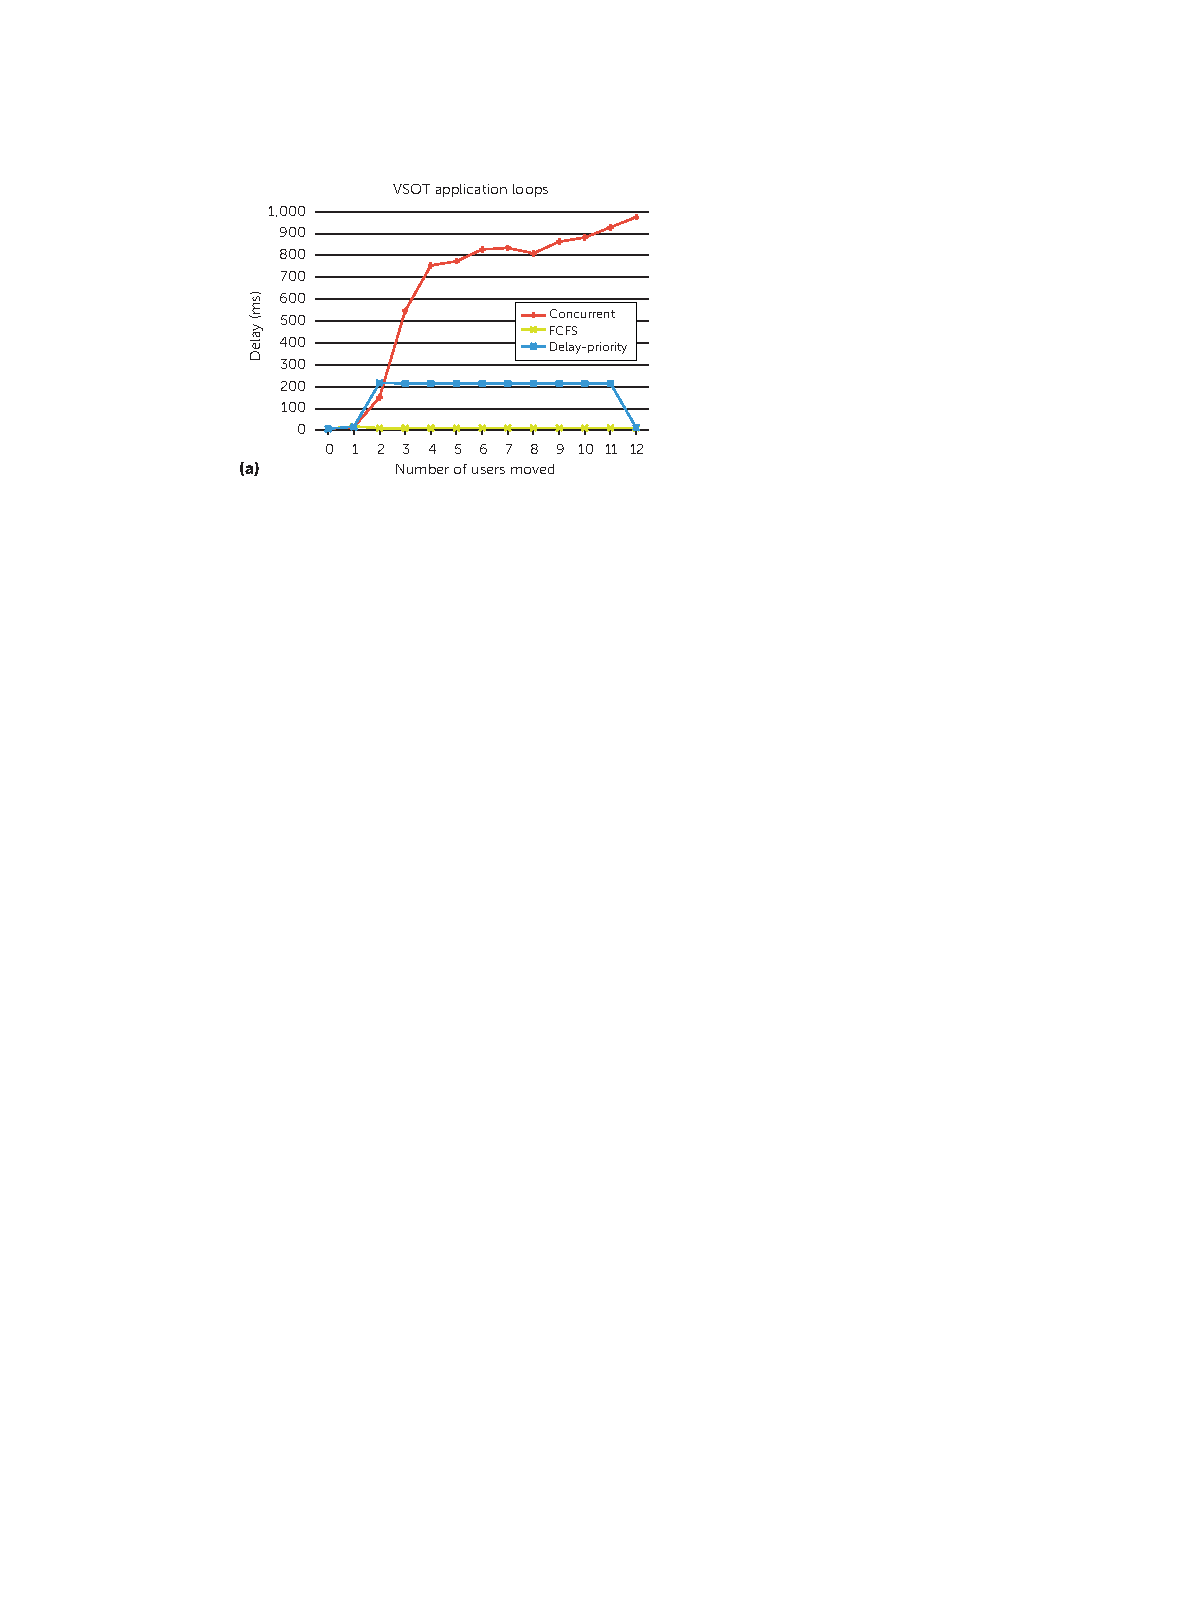
\includegraphics[scale=1.2]{images/4a.pdf}}
 		\caption[]{}
 	\end{figure}
\end{frame}

\begin{frame}
 	\begin{figure}[htbp]
 		\centerline{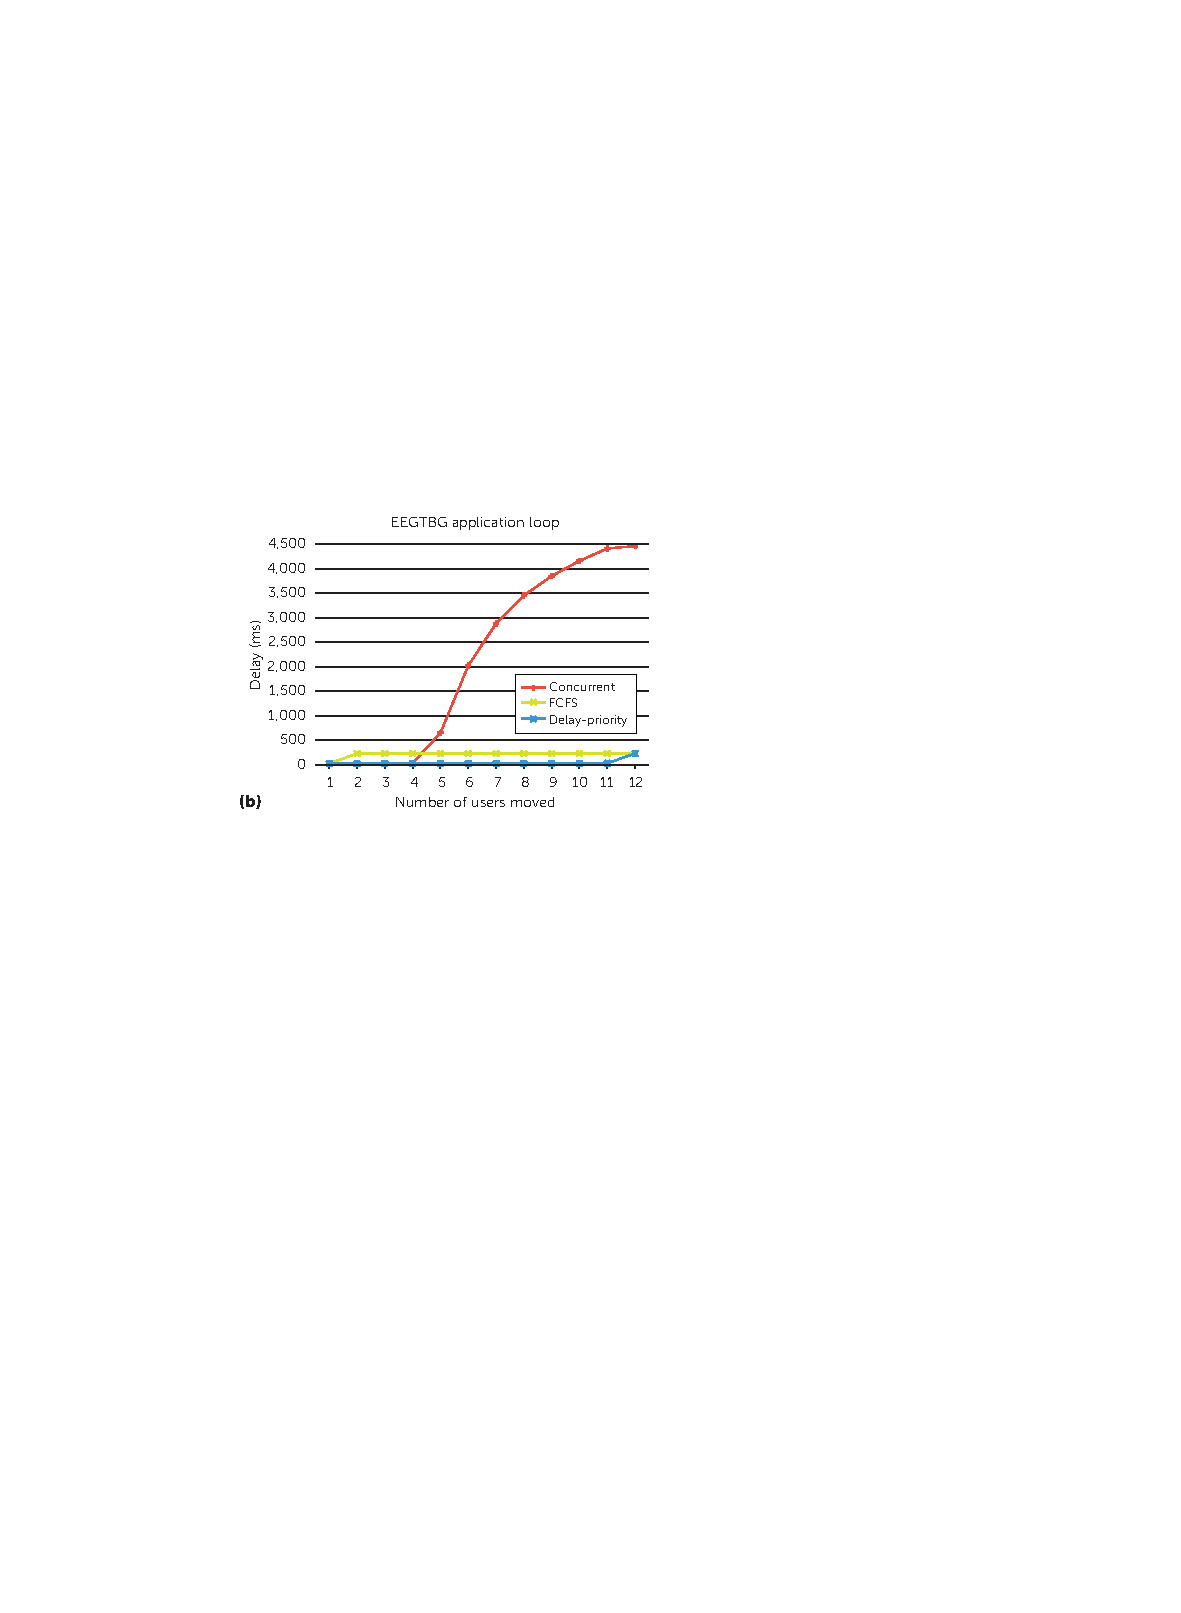
\includegraphics[scale=1.2]{images/4b.pdf}}
 		\caption[]{}
 	\end{figure}
\end{frame}

\begin{frame}
 	\begin{figure}[htbp]
 		\centerline{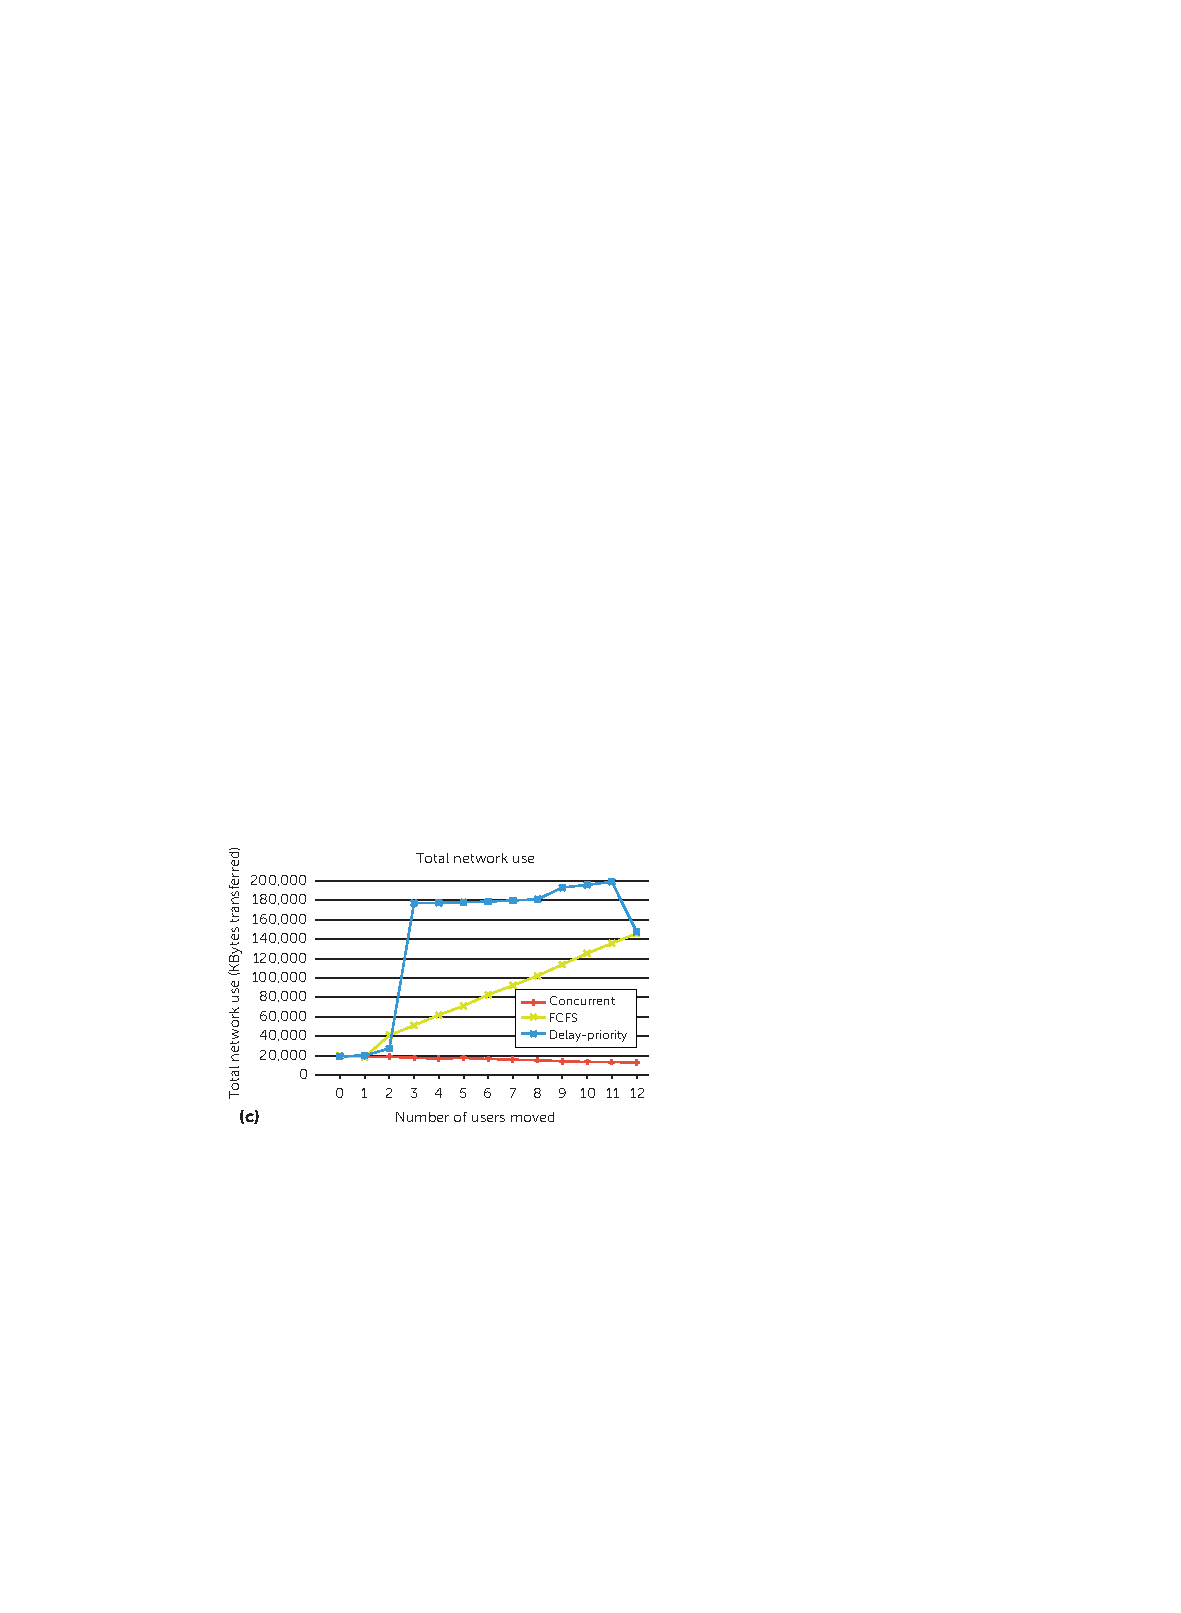
\includegraphics[scale=1.2]{images/4c.pdf}}
 		\caption[]{}
 	\end{figure}
\end{frame}

\begin{frame}
 	\begin{figure}[htbp]
 		\centerline{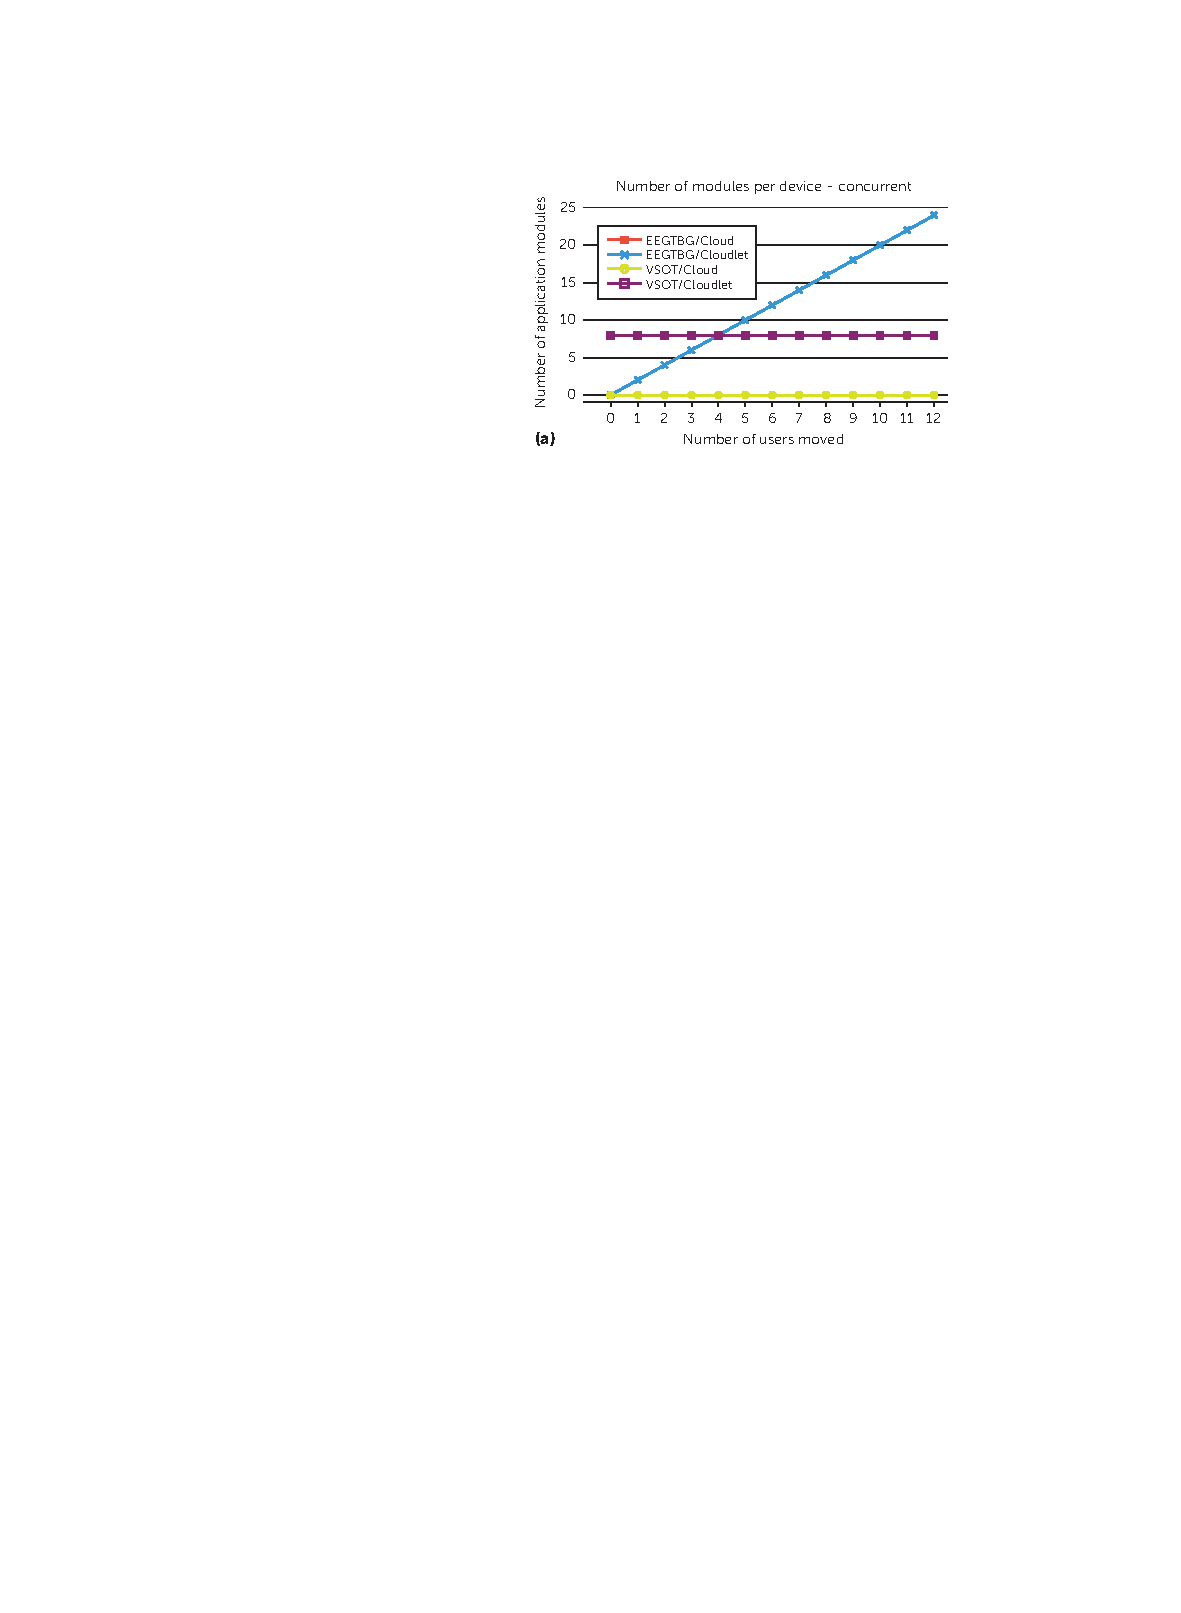
\includegraphics[scale=1.2]{images/5a.pdf}}
 		\caption[]{}
 	\end{figure}
\end{frame}

\begin{frame}
 	\begin{figure}[htbp]
 		\centerline{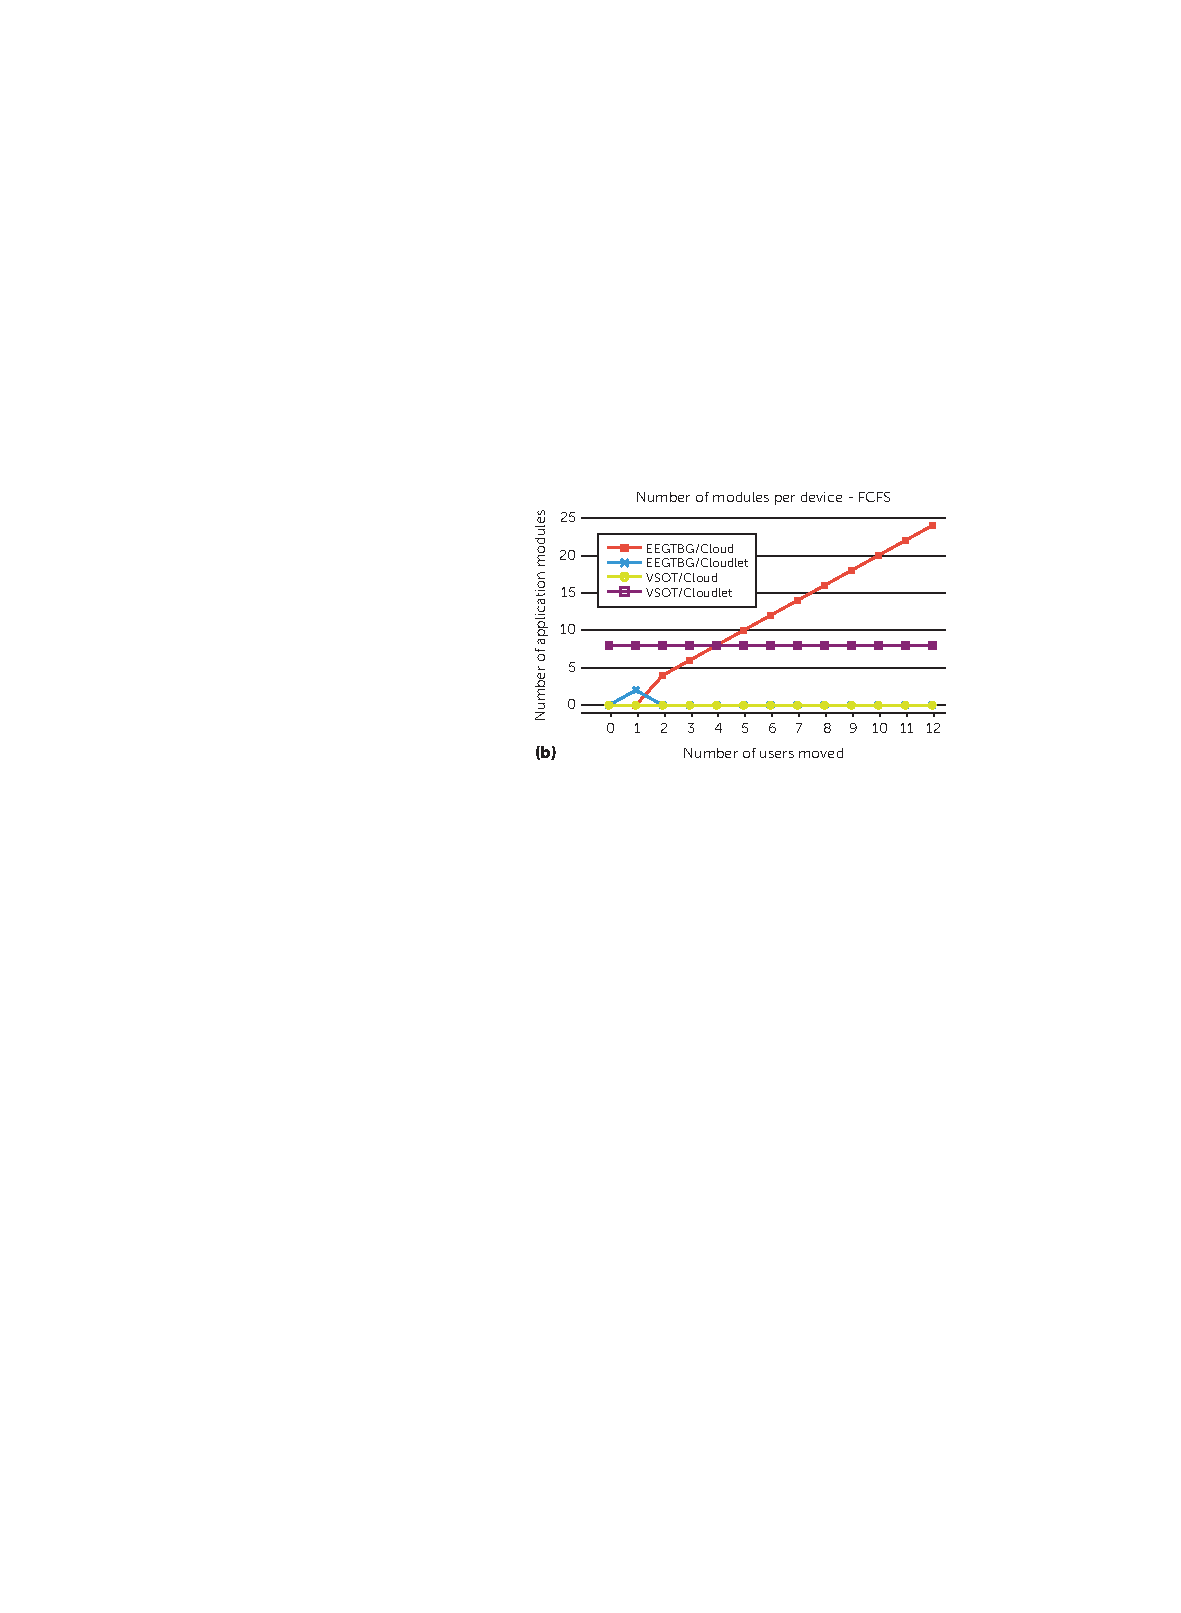
\includegraphics[scale=1.2]{images/5b.pdf}}
 		\caption[]{}
 	\end{figure}
\end{frame}

\begin{frame}
 	\begin{figure}[htbp]
 		\centerline{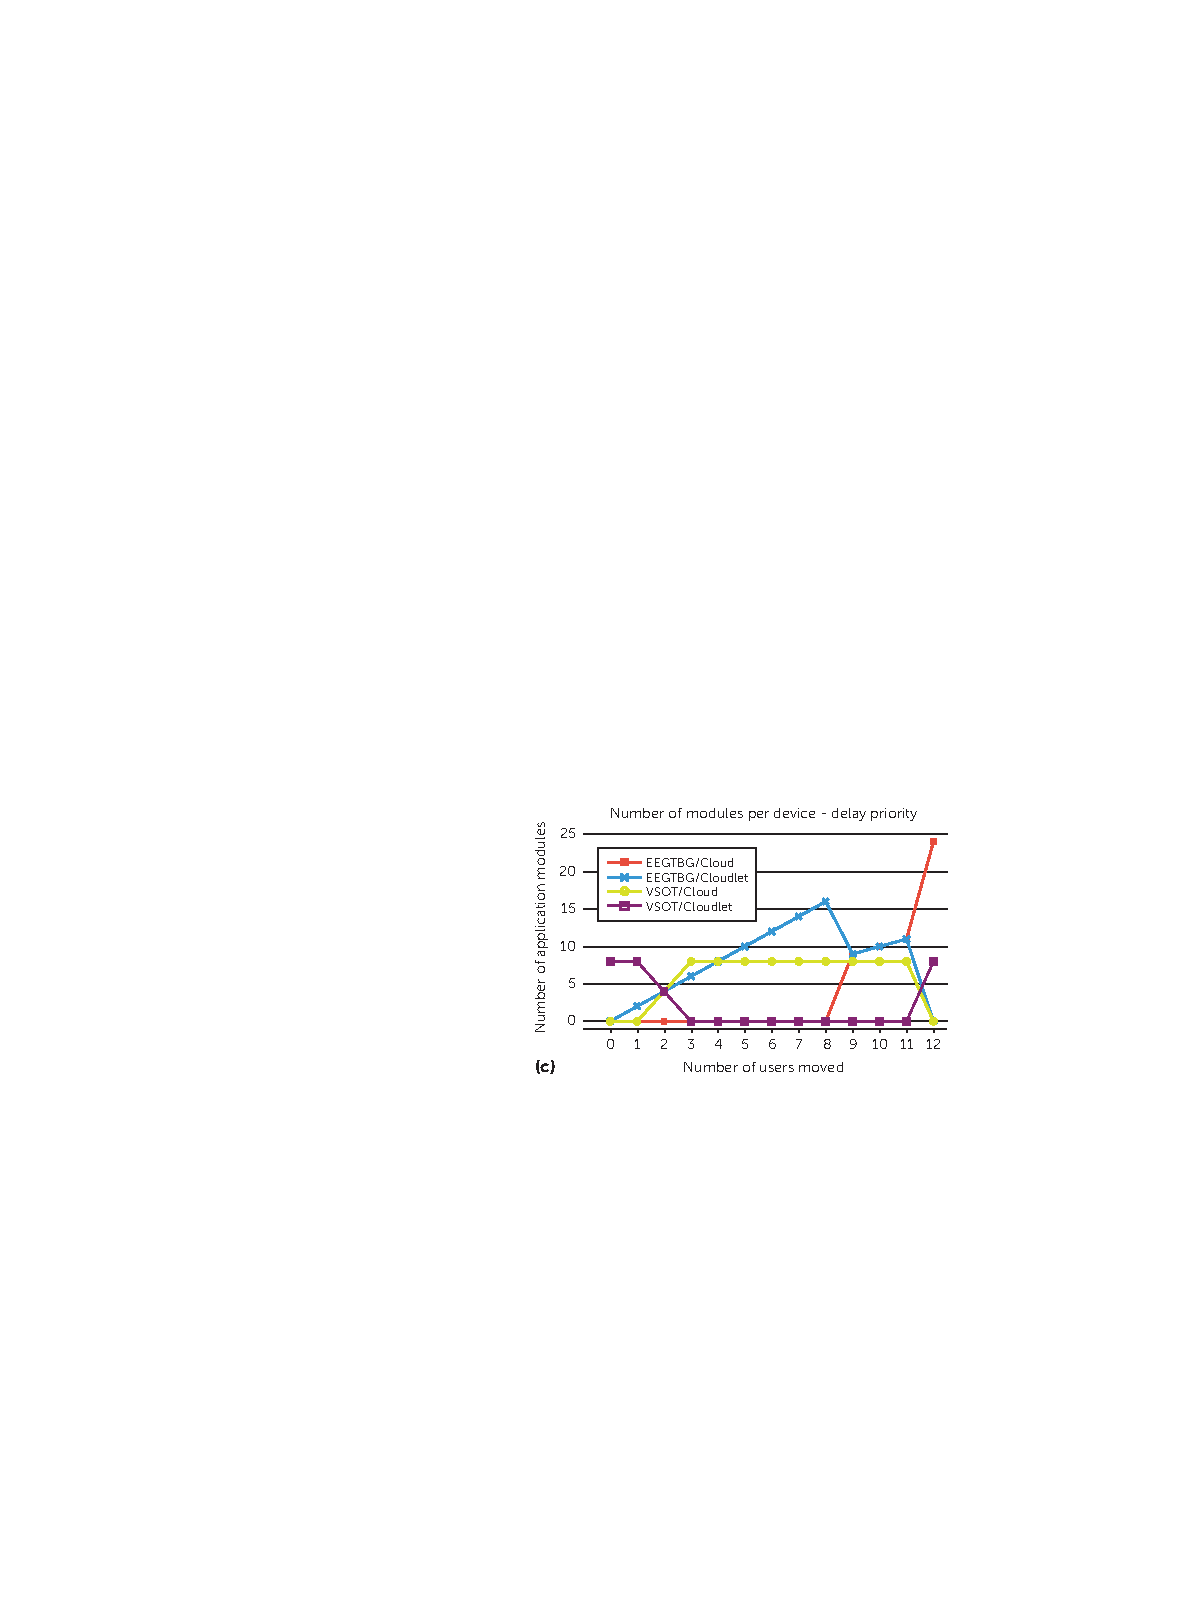
\includegraphics[scale=1.2]{images/5c.pdf}}
 		\caption[]{}
 	\end{figure}
\end{frame}

\section[Challenges and Future Directions]{Challenges and Future Directions}

\begin{frame}
	\tableofcontents[currentsection]
\end{frame}

\begin{frame}
	\frametitle{Challenges and Future Directions}
\end{frame}

\section[Conclusions]{Conclusions}

\begin{frame}
	\tableofcontents[currentsection]
\end{frame}

\begin{frame}
	\frametitle{Conclusions}
% 	\begin{block}{}
% 		\begin{itemize}
% 			\item[•] Revisão das questões de seleção de serviços em nuvam, considerando diferentes abordagens CSB;
% 			\newline
% 			\item[•] Nenhuma abordagem investigada suporta todos os atributos propostos para um CSB efetivo; 
% 		\end{itemize}
% 	\end{block}
\end{frame}

\begin{frame}
	\frametitle{Summary and Conclusions}
% 	\begin{block}{}
% 		\begin{itemize}
% 			\item[•] Na teoria é possível, porém, torna-se impraticável um CSB que suporte todos os atributos;
% 			\newline
% 			\item[•] É necessário priorizar os atributos a fim de encontar um equilíbrio e selecionar os que melhor se conformam ao objetivo do CSB.
% 		\end{itemize}
% 	\end{block}
\end{frame}

% \begin{frame}{Dados do Artigo}
% \begin{minipage}{0.47\textwidth}
% 		\begin{itemize}
% 			\item[•] Accepted Date: 10/05/2017
% 			\item[•] Online Date: 13/06/2018
% 			\item[•] FI 2017: 1.105 (\textit{journal})
% 		\end{itemize}
% \end{minipage}
% \begin{minipage}{0.5\textwidth}
%     \begin{figure}[htbp]
% 		\centerline{
\includegraphics[scale=0.15]{images/fcs.jpg}}
% 			\label{fig:consolidatarefas6}
% 		\end{figure}
% \end{minipage}
% Acesso: \url{http://journal.hep.com.cn/fcs/EN/10.1007/s11704-017-6124-7}
% \end{frame}

%\section{Referências}
%
%\begin{frame}
%	\tableofcontents[currentsection]
%\end{frame}
%
%\begin{frame}[allowframebreaks]
%	\frametitle{Referências}
%	\def\newblock{}
%	\bibliographystyle{plain}
%	\tiny \bibliography{bibliografia}
%\end{frame}

% \section*{Agradecimentos}
	
% \begin{frame}
% 	\begin{center}
% 		\textbf{Obrigado!}
% 	\end{center}
% 	\begin{figure}[htbp]
% 		\begin{center}
% 			
\includegraphics[scale=.09]{images/Question-Mark.jpg}
% 		\end{center}
% 	\end{figure}
% 	\begin{center}
% 		\url{madsantos@inf.ufpel.edu.br}
% 	\end{center}
% \end{frame}

%%%%%%%%%%%%%%%%%%%%%%%%%%%%%%%%%%%%%%%%%%%%
% Último Slide
%%%%%%%%%%%%%%%%%%%%%%%%%%%%%%%%%%%%%%%%%%%%
\frame
{
	\pgfdeclareimage[height=1.5cm]{logo}{images/lups_oficial.png}
	\logo{\pgfuseimage{logo}
}	
	\logo{\vspace{3mm} 
	\begin{large}
		\textbf{Obrigado!} 
	\end{large}}
	\titlepage
}

\end{document}